\documentclass[10pt,twoside]{report}
\usepackage{charter,titlesec,fancyhdr,wrapfig,framed}
\usepackage[pdftex]{graphicx}
\usepackage{colortbl}
\definecolor{white}{gray}{1.0}
\definecolor{gray-5}{gray}{0.95}
\definecolor{gray-10}{gray}{0.9}
\definecolor{gray-20}{gray}{0.8}
\definecolor{gray-30}{gray}{0.7}
\definecolor{gray-40}{gray}{0.6}
\definecolor{fadered}{rgb}{0.8824, 0.9529, 0.8745}
\usepackage{subfigure}
\usepackage[papersize={6.8in,8.8in},left=2cm,right=2cm,top=3cm,bottom=2cm]{geometry}
\usepackage{setspace}
\usepackage[charter]{mathdesign}
\usepackage[small]{caption}
\usepackage[scaled]{beramono}
\usepackage{abstract}
\usepackage{nextpage}
\usepackage{picins}

\usepackage{listings} 
%\lstset{numbers=left, numberstyle=\scriptsize\ttfamily, numbersep=8pt, captionpos=b} 
\lstset{backgroundcolor=\color{gray-5}}
\lstset{basicstyle=\small\ttfamily}
\lstset{framesep=4pt, frame=single, framerule=0pt, tabsize=4}
\lstset{language={}}
\newcommand{\inlineCode}{\lstinline[basicstyle=\small\ttfamily, backgroundcolor=\color{white}, breaklines=true]}

\usepackage[colorlinks=true,linkcolor=black,citecolor=black,urlcolor=black,filecolor=black,bookmarks=true]{hyperref}
\hypersetup{
pdfauthor = {Michael Specht},
pdftitle = {Proteomatic},
pdfsubject = {},
pdfkeywords = {},
pdfcreator = {LaTeX},
pdfproducer = {pdflatex}}
\renewcommand{\figurename}{Fig.}

%\usepackage{eso-pic}
\usepackage{color}
\usepackage{type1cm}
\makeatletter
  \AddToShipoutPicture{%
    \setlength{\@tempdimb}{.5\paperwidth}%
    \setlength{\@tempdimc}{.5\paperheight}%
    \setlength{\unitlength}{1pt}%
    \put(\strip@pt\@tempdimb,\strip@pt\@tempdimc){%
      \makebox(0,0){\rotatebox{12}{\textcolor[gray]{0.86}{
        \fontsize{2.4cm}{2.4cm}\selectfont{preliminary \linebreak copy}}}}
    }
}
\makeatother


\include{chapterleft}
\fboxsep0pt
\fboxrule0.05pt

\newcommand{\image}[5]{
  \begin{figure}[htbp]
    \centering
    \includegraphics[width=#3\textwidth]{#2}
    \caption[#5]{#4}
    \label{fig:#1}
  \end{figure}
}

\newcommand{\imageFrame}[5]{
  \begin{figure}[htbp]
    \centering
    \fbox{
      \includegraphics[width=#3\textwidth]{#2}
    }
    \caption[#5]{#4}
    \label{fig:#1}
  \end{figure}
}


\setlength{\parskip}{2mm}
\setlength{\parindent}{0mm}
\renewcommand{\baselinestretch}{1.2} 
\renewcommand{\arraystretch}{1.2} 
\tolerance=2000

\renewcommand{\headrulewidth}{0.25pt}

\pagestyle{fancy}

\renewcommand{\chaptermark}[1]{\markboth{#1}{}}
\renewcommand{\sectionmark}[1]{\markright{#1}}

%\setlength{\marginparwidth}{1.5cm}
%\newcommand{\note}[1]{\marginpar{\color{gray-40}\footnotesize \flushleft #1}}
\newcommand{\note}[1]{}

\newcommand{\imageCourtesy}[2]{Image courtesy of #1 \cite{#2}.}

\fancyhf{}
\fancyhead[EL,OR]{\thepage}
\fancyhead[ER]{\leftmark}
\fancyhead[OL]{\rightmark}
\fancypagestyle{plain} {
  \fancyhf{}
  \renewcommand{\headrulewidth}{0pt}
}

\lstnewenvironment{todo}{\lstset{numbers=none,frame=none,backgroundcolor=\color{fadered}}}{}

\begin{document}

\pagestyle{empty}
\begin{titlepage}
\begin{center}
%\normalfont\noindent\bf\Huge{Interactive Glyph-based 3D Visualization \linebreak of
%Dynamic PET Datasets}
\vspace*{2cm}
\normalfont\noindent\bf\Huge{Proteomatic}  \\
\vspace*{0.5cm}
\normalfont
\Large{User's Guide and} \\
\Large{Developer's Reference Manual}

\vfill

\normalfont\noindent\large{}
\end{center}
\end{titlepage}

\cleartoevenpage
\setcounter{page}{2}
\setcounter{tocdepth}{1}
\setcounter{secnumdepth}{2}
\tableofcontents
\newpage

\thispagestyle{empty}

%\cleardoublepage
\pagestyle{fancy}

\fancypagestyle{plain} {
  \renewcommand{\headrulewidth}{0.25pt}
  \fancyhf{}
  \fancyhead[EL,OR]{\thepage}
}
\cleartoevenpage

\chapter{User's Guide}
\newpage




\section{Introduction}



	\piccaption{The Proteomatic main window.}\parpic[r]{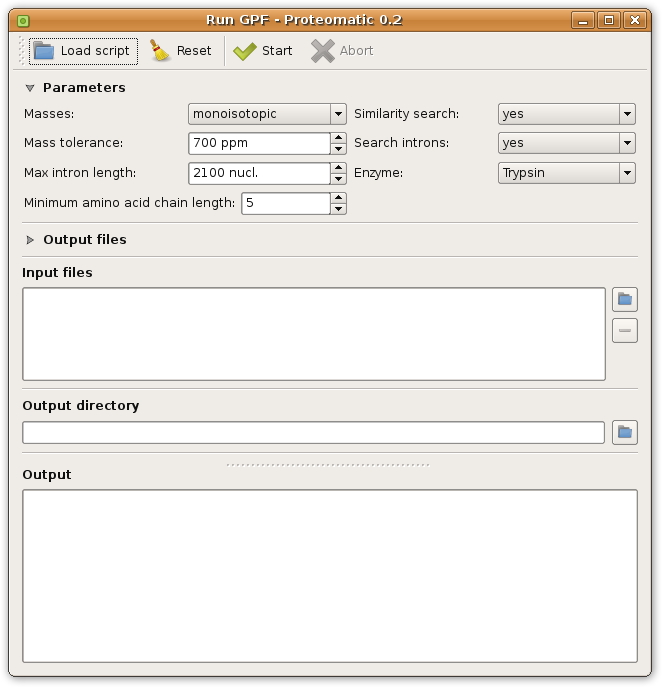
\includegraphics[width=0.5\textwidth]{images/proteomatic.jpg}} 

Proteomatic is the Proteomics researcher's swiss army knife. It enables a user to try out freely available open source tools by automatically downloading and installing these tools and providing a uniform user interface to configure and run them (commercial tools can be used as well but require manual configuration).

Furthermore, tools can be chained together to form a pipeline. Proteomatic is availble on various platforms including Linux, Mac OS and Windows.

Proteomatic originated from the following observations:

\begin{enumerate}
\item {\bf Increasing availability of open source tools.} More and more proteomics open source software tools are becoming available. In many cases, these programs are implemented as command line tools, which scares off biologists who are not used to working with the command line. Also, these tools often have lots of parameters, which must be manually adjusted and tried out in order to achieve good results.
\item {\bf Increased automation and high-throughput proteomics.} ...
\end{enumerate}

	\piccaption{Information flow for the OMSSA wrapper script.}\parpic[r]{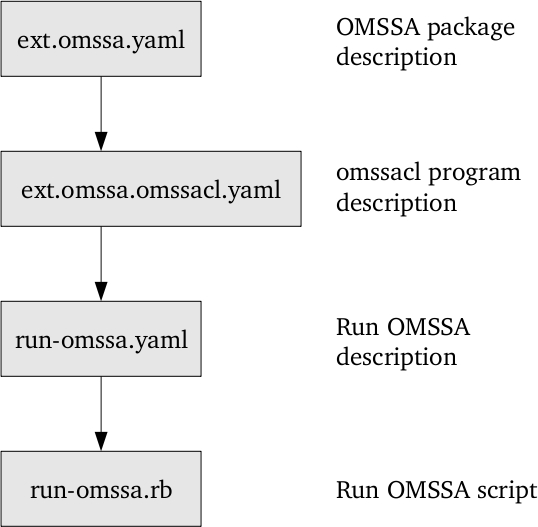
\includegraphics[width=0.5\textwidth]{images/scripts-and-descriptions.jpg}} 

The Proteomatic answer to the points stated above is a collection of scripts which encapsulate both open source and commercial software or implement miscellaneous functionality. Each script has a formal description which contains the title, description, and the parameters, along with their descriptions and default values, of the script. If a script acts as a wrapper for an external program, it will include the parameters for this program which are taken from its description.

In addition to scripts and external programs, file types are described as well, which makes it possible to chain scripts together to form a processing pipeline.

On top of this (command line) script layer, a user friendly GUI can be used to load, configure and run these scripts.

\cleartoevenpage

\chapter{Developer's Reference Manual}
\newpage




\section{Scripts}



Proteomatic scripts come in two flavors: {\em processors} and {\em converters}. A processor script takes a number of input files and parameters and then writes a number of output files that result from {\em processing} the given input files. A converter script, on the other hand, takes each input files and {\em converts} it to a corresponding output file, regardless of the other input files, but also taking parameters into account.

Reagrdless of its type, a Proteomatic script consists of two parts:

\begin{enumerate}
\item {\bf The script description.} This YAML file contains the title, description and options of the script.
\end{enumerate}

\begin{enumerate}
\item {\bf The script.} This file contains Ruby code.
\end{enumerate}



\subsection{Processor scripts}



The filename of the script description file is \inlineCode�scripts/include/properties/example.yaml�. It contains a YAML formatted description.


\begin{lstlisting}
title: Example script

type: processor

group: Some sub menu/Another sub menu  # this will appear in the GUI script menu

input:
  - key: peptides                      # all files from this group can be
                                       # accessed with @input[:peptides]
    label: Peptides                    # this will be useful for the GUI
    formats: [txt]                     # a list of valid formats for this group
                                       # (file formats must be defined, too)
    min: 1                             # min and max file counts can be specified

defaultOutputDirectory: peptides       # by default, the output files go to the
                                       # directory of the first file of the group
                                       # specified here

output:                                # each entry described an output file that
  - key: peptideMasses                 # can be enabled or disabled by the user
    label: Peptide and fragment masses # (some result files may be uninteresting
    format: html                       # in some cases)
    filename: peptide-masses.html
    default: yes
  - key: msPeptideMasses               # if the users wants this file, then
                                       # @output[:msPeptideMasses] will contain
                                       # the full path to the output file
    label: MS peptide masses           # this will be useful for the GUI
    format: txt                        # the format of this output file, important
                                       # for pipeline construction
    filename: ms-peptide-masses.txt    # the filename of this output file, can be
                                       # prefixed by the user
    default: yes                       # whether the file should be written by default
\end{lstlisting}


The filename of the script file is \inlineCode�scripts/example.rb�. The skeleton of a Proteomatic script looks like this:


\begin{lstlisting}
require 'include/proteomatic'

class Example < ProteomaticScript
	def run()
	end
end

lk_Object = Example.new
\end{lstlisting}


The \inlineCode�require 'include/proteomatic'� must be the first line. Then, a subclass of \inlineCode�ProteomaticScript� is defined which is instanciated as \inlineCode�lk_Object� after that. Within the \inlineCode�run� method, several member variables can be accessed:

\begin{enumerate}
\item {\bf Input files.}
\end{enumerate}



For processor scripts, all input files are stored in the \inlineCode�@input� hash, which has an array of absolute input file paths for each input group key.




\begin{enumerate}
\item {\bf Output files.}
\end{enumerate}



For processor scripts, ... yar de yar yar.




And there's even more!



\section{External tools}



Tools can be added, too! ``{\bf Wow}'', you say.
\end{document}
